% !TEX root = main.tex

\section{中文分词}
最大匹配法:有一个词典,设定最大词长,做字符串匹配
\begin{figure}[H]
\centering
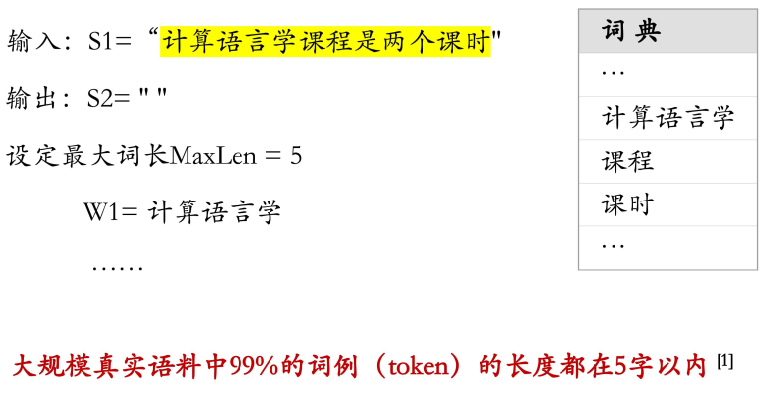
\includegraphics[width=0.8\linewidth]{fig/max_matching.png}
\end{figure}

最优路径法:
\begin{itemize}
\item 选择一条词数最少的路径
\item 半词法分词(加权)
\item 最大概率法:在词图上选择词串概率最大的分词路径(动态规划)
\[\max(P(W_1\mid S),P(W_2\mid S))\]
\end{itemize}
\begin{figure}[H]
\centering
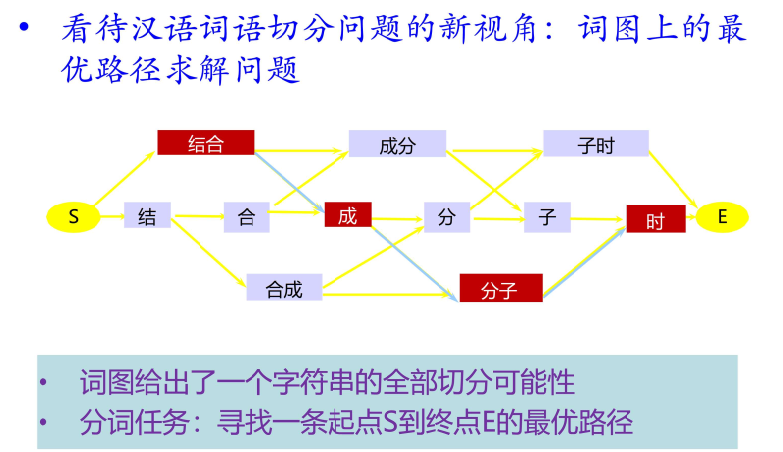
\includegraphics[width=0.8\linewidth]{fig/best_path.png}
\end{figure}

基于字序列标注的方法
\begin{figure}[H]
\centering
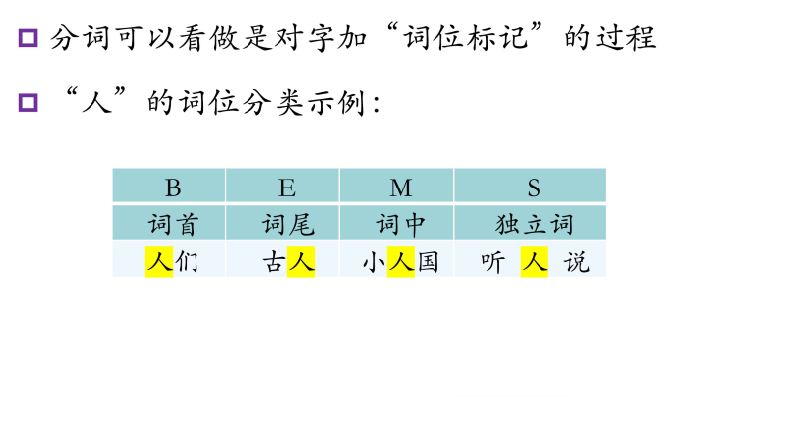
\includegraphics[width=0.8\linewidth]{fig/word_pos_labeling.png}
\end{figure}